\documentclass[12pt]{exam}

\usepackage[utf8]{inputenc}  % For UTF8 source encoding.
\usepackage{amsmath}  % For displaying math equations.
\usepackage{amsfonts} % For mathematical fonts (like \mathbb{E}!).
\usepackage{upgreek}  % For upright Greek letters, such as \upvarphi.
\usepackage{wasysym}  % For additional glyphs (like \smiley!).
\usepackage{mathrsfs} % For script text (hash families and universes).
\usepackage{enumitem}
\usepackage{graphicx}
% For document margins.
\usepackage[left=.8in, right=.8in, top=1in, bottom=1in]{geometry}
\usepackage{lastpage} % For a reference to the number of pages.
\usepackage[table,xcdraw]{xcolor}
\usepackage{pdfpages}
\usepackage{verbatim}

% TODO: Enter your name here :)
\newcommand*{\authorname}{Luis A. Perez}

\newcommand*{\duedate}{Wednesday, July 20th}
\newcommand*{\duetime}{11:59 pm}

% Fancy headers and footers
\headrule
\firstpageheader{EE 263\\Summer 2019}{Midterm \\ }{Due: \duedate\\at \duetime}
\runningheader{EE 263}{Midterm}{\authorname}
\footer{}{\footnotesize{Page \thepage\ of \pageref{LastPage}}}{}

% Exam questions.
\newcommand{\Q}[1]{\question{\large{\textbf{#1}}}}
\qformat{}  % Remove formatting from exam questions.

% Useful macro commands.
\newcommand*{\bigtheta}[1]{\Theta\left( #1 \right)}
\newcommand*{\bigo}[1]{O \left( #1 \right)}
\newcommand*{\bigomega}[1]{\Omega \left( #1 \right)}
\newcommand*{\prob}[1]{\text{Pr} \left[ #1 \right]}
\newcommand*{\ex}[1]{\text{E} \left[ #1 \right]}
\newcommand*{\var}[1]{\text{Var} \left[ #1 \right]}

\newcommand*{\norm}[1]{\left\lVert #1 \right\rVert}
\newcommand*{\HH}{\mathscr{H}}   % Family of hash functions.
\newcommand*{\UU}{\mathscr{U}}   % Universe.
\newcommand*{\eps}{\varepsilon}  % Epsilon.


% Custom formatting for problem parts.
\renewcommand{\thepartno}{\roman{partno}}
\renewcommand{\partlabel}{\thepartno.}

% Framed answers.
\newcommand{\answerbox}[1]{
\begin{framed}
\hspace{\fill}
\vspace{#1}
\end{framed}}

\printanswers

\setlength\answerlinelength{2in} \setlength\answerskip{0.3in}

\begin{document}
\title{EE 263 Midterm}
\author{\authorname}
\date{}
\maketitle
\thispagestyle{headandfoot}
\setcounter{MaxMatrixCols}{15}

\begin{questions}
%%%%%%%%%%%%%%%%%%%%%%%%%%%%%%%%%%%
\Q{Fitting a model for hourly temperature}

  \begin{solution}
    \begin{enumerate}[label=(\alph*)]
      \item Let our capture image be $Y = \begin{pmatrix} y_1 & \cdots & y_N \end{pmatrix} \in \mathbb{R}^{2 \times N}$. The rotation by angle $\theta$ and positive $\alpha > 0$ for face $i$ would correspond to the operation:
      \[
        Y = RF^{(i)}
      \]
      So the tasks consists of finding the $i$ for which the above equation holds. The other complicating aspect is that we don't know $R$. However, we propose the following algorithm to find a candidate matrix $\mathbb{R}$.

      \begin{itemize}
        \item Take the $j$-th facial feature from the $i$-th example, $z_1 = F_j^{i} \in \mathbb{R}^2$ and the corresponding facial feature of our output face, $z_2 = Y_j \in \mathbb{R}^2$ (these are just the $j$-th columns of $F^{i}$ and $Y$). 
        \item Find a rotation and scaling matrix $\hat{R}$ between these two vectors, $z_1, z_2$. Note that this is possible as long as these two vectors are non-zero. However, in the case where $z_1 = 0, z_2 \neq 0$, no transformation exists, and if $z_1 \neq 0, z_2 = 0$, the only possible transformation is $\hat{R} = 0$ (the zero-matrix). Lastly, if both are $0$, then the trivial must have $\hat{R} = I$. 

        As such, for the cases where we know both $z_1 \neq 0, z_2 \neq 0$, we know that $z_1$ can always be transformed into $z_2$ by rotating and scaling. In more detail. to find this candidate matrix $\hat{R}$, we need to know (1) the scaling factor $\alpha$ and (2) the angle of rotation $\theta$. We have:
         \[
          \alpha = \left| \frac{||z_2||}{||z_1||} \right|
         \]
         since it is just the ratio of the legths. The angle of rotation is just slightly trickier, but can be computed using the following relation
         \[
          \theta = \cos^{-1} \left(\frac{z_2^Tz_1}{||z_1||||z_2||}\right)
         \]
         Note that this actually gives us two candidate angles, the other being $2\pi - \theta$. With this information, we can construct two candidate rotation/scaling matrices $\hat{R}_1$ and $\hat{R}_2$. To select the correct one, we simply try both and find the $k$ such that:
         \[ 
          Y_j = \hat{R}_kF^{(i)}_j
         \]
         holds.
         \item Now that we've narrowed it down to a single $\hat{R}$ candidate matrix, we just check if
         \[
          Y = \hat{R}F^{(i)}
         \]
         If the above hold, we are done, and have found that the $i$-th example face corresponds to the capture face. If it does not hold, we continue tot he next example face.
      \end{itemize}
      \item We apply the above method (see attached code). We find that $Y_{\text{rot}}$ corresponds to $F_2$.
      \item
        Minmizing $\rho$ correspond to minimizing the objective function:
        \[
          J = \sum_{i=1}^N ||y_i - Rx_i^{(k)} - t||^2
         \]
        We focus first on finding the optimal value of $t$. We can do this by taking the derivative with respect to $t$ and setting equal to $0$, which is straight-forward. We have:
        \begin{align*}
          -2 \sum_{i=1}^N (y_i - Rx_i^{(k)} - t) &= 0 \\
          \implies \sum_{i=1}^N y_i - R\sum_{i=1}^N x_i^{(k)} &= tN \\
          \implies t &= \frac{1}{N} \sum_{i=1}^N y_i - R \frac{1}{N}\sum_{i=1}^{N} x_i^{k} \\
          &= \bar{y} - R\bar{x}
        \end{align*}

       where:
       \begin{align*}
        \bar{x} &=  \frac{1}{N} \sum_{i=1}^N x_i^{(k)} \\
        \bar{y} &= \frac{1}{N} \sum_{i=1}^N y_i
       \end{align*}
       Plugging this optimal value of $t$ into our objective, we have:
       \[
          J = \sum_{i=1}^N ||y_i - Rx_i^{(k)} - \bar{y} + R\bar{x}||^2 = \sum_{i=1}^N ||(y_i - \bar{y}) - R(x_i^{(k)} -\bar{x})||^2
       \]
       So with this transformation, the problem once again just becomes finding the optimal scaling and rotation matrix $R$ to find the given data (and minimize the objective) where we have $\tilde{y}_i = y_i - \bar{y}$ and $\tilde{x}_i = x_i^{(k)} - \bar{x}$.


       As such, focusing on this new problem of estimating $R$ to minimize the above, let us see if we can simplify. We have $R = \alpha R'$ where $R'$ is orthonormal. We have:
       \begin{align*}
        ||\tilde{y}_i - \alpha R'\tilde{x}_i^{(k)}||^2 &= (\tilde{y}_i - \alpha R'\tilde{x}_i)^T(\tilde{y}_i - \alpha R'\tilde{x}_i) \\
        &=\tilde{y}_i^T\tilde{y}_i + \alpha^2 \tilde{x}_i^TR'^TR'\tilde{x}_i - 2\alpha \tilde{y}_i^TR'\tilde{x}_i \tag{Last term is scalar, so $a^T =a $} \\
        &= \tilde{y}_i^T\tilde{y}_i + \alpha^2 \tilde{x}_i^T\tilde{x}_i - 2\alpha \tilde{y}_i^TR'\tilde{x}_i \tag{$R'^TR' = I$} 
       \end{align*}
       Since we're trying to minimize this with respect to $R'$, our minimization can be simplified greatly (the first two terms above don't depend on $R'$) and we can drop scalars. As such, we have our new objective the maximization of:
       \[
        \sum_{i=1}^N \tilde{y}_i^TR'\tilde{x}_i
       \]
       We can rewrite the above entirely in matrix notation as:
       \[
        \text{trace} (Y^TR'X) = \text{trace}{R'XY^T}
       \]
       Then computing the singular-value decomposition of $S = XY^T = U\Sigma V^T$, we have:
       \[
        \text{trace}(R'XY^T) = \text{trace}(R'U\Sigma V^T) = \text{trace}{\Sigma V^T R' U}
       \]
       IN this last step, let us note that $V,R'$ and $U$ are all orthogonal matrices (by definition of rotation and by SVD), as such, we have $(V^TRU)_{ij} \leq 1$. This means that the only way to maximize the above objective (by manipulating $R'$), racalling that $\Sigma$ is a diagonal with non-negative entries, is to have the diaginal entries of $(V^TR'U)_{ii} = 1$, which implies the following:
       \begin{align*}
        I &= V^TR'U \\
        \implies R' = VU^T \tag{Inverse of orthonormal matrices is transpose}
       \end{align*}
       We know have a formula for computing $R'$ and $t$. The only variable left to figure out is $\alpha$. Going back to our simplified objective, we are now trying to minimize:
       \[
        \alpha^2\sum_{i=1}^n \tilde{x}_i^T\tilde{x}_i - 2\alpha \sum_{i=1}^N \tilde{y}_i^T R' \tilde{x}_i
       \]
       Taking the derivative with respect to $\alpha$ and setting equal to zero, we have:
       \begin{align*}
        2\alpha \sum_{i=1}^N \tilde{x}_i^T\tilde{x}_i &= 2\sum_{i=1}^N \tilde{y}_i^TR'\tilde{x}_i \\
        \implies \alpha &= \frac{\sum_{i=1}^N \tilde{y}_i^TR'\tilde{x}_i}{\sum_{i=1}^N \tilde{x}_i^T\tilde{x}_i}
       \end{align*}
      With the above, we have completed the process of finding all the required parameters.
      \item See the attached code for details. These are the results:

      Scale rotation + translation estimates for $F_1$
      \begin{verbatim}
        R = [[ 1.38710025 -0.50402031]
         [ 0.50402031  1.38710025]]
        t = [[0.26475362]
         [0.07103614]]
      \end{verbatim}
        Scale rotation + translation estimates for $F_2$
        \begin{verbatim}
        R = [[ 1.36865856 -0.49728905]
         [ 0.49728905  1.36865856]]
        t = [[0.27399331]
         [0.04565355]]
        \end{verbatim}
        Scale rotation + translation estimates for $F_3$
        \begin{verbatim}
        R = [[ 1.38049264 -0.49966651]
         [ 0.49966651  1.38049264]]
        t = [[0.27343758]
         [0.05007972]]
        \end{verbatim}
        Scale rotation + translation estimates for $F_4$
        \begin{verbatim}
        R = [[ 1.42094548 -0.5162301 ]
         [ 0.5162301   1.42094548]]
        t = [[0.25391536]
         [0.10100179]]
        \end{verbatim}
        Scale rotation + translation estimates for $F_5$
        \begin{verbatim}
        R = [[ 1.33411965 -0.48425504]
         [ 0.48425504  1.33411965]]
        t = [[0.27703282]
         [0.03803171]]
        \end{verbatim}

      We now have the RMSEs:
        \begin{itemize}
          \item RMSE for $F_1$ is 1.215783026538849
          \item RMSE for $F_2$ is 1.202885795582196
          \item RMSE for $F_3$ is 1.2080822140116791
          \item RMSE for $F_4$ is 1.2321052401027686
          \item RMSE for $F_5$ is 1.1978958153633974
        \end{itemize}
      \item The method used in part (b) actually requires a lower decimal point precission, since it involves no inversion of calculation of matrix decompositions. In fact, the method in part (b) was selected with the explicit knowledge that no noise would be found in the image, and as such, we could take advantage of that.

      As for the method in part (d), this also does not rely on matrix inversion (which would throw our condition value quite high for the matrices). Instead, we're taking advange of the fact that what we want is a rotation matrix, and can therefore make use of SVD, which has lower precision requirements compared to matrix inversion.

      See attached code for the figure.
    \end{enumerate}
  \end{solution}

\begin{solution}
  \begin{enumerate}[label=(\alph*)]
    \item For the weighed least squares problem, we know that we can actualy rewrite the objective back into matrix form. Our objective is:
    \[
      \sum_{i=1}^n w_i(\tilde{a}_i^T x - y_i)^2 = \sum_{i=1}^n (\sqrt{w_i}\tilde{a}_i^T x - \sqrt{w_i}y_i)^2 
    \]
    The above can be written in the form:
    $$
      ||WAx - Wa ||_2^2
    $$
    where the matrix $W \in \mathbb{R}^{m \times m}$ is given by:
    \[
      W =
        \begin{bmatrix}
          w_1 & 0 & \cdots & 0 \\
          0 & w_2 & \cdots & 0 \\
          0 & 0 & \ddots & 0 \\
          0 & 0  & \cdots & w_m
        \end{bmatrix}
    \]

    Where $w_i$ lies in the diagonal. For convenience, we define $\sqrt{W}$ as the matrix $W$ where each diagonal entry has been square-rooted. Since the $w_i$ are given, we can just consider these to be part of our system (eg, consider $\sqrt{W}A$ as $\tilde{A}$ and $\sqrt{W}y$ as $\tilde{y}$, the output of our system).

    With the phrasing, as long as $\sqrt{W}A$ is also skinny and full-rank (and given that $A$ is skinny and full rank, the only additional requirement would be that $W$ be full-rank). Since $W$ is a diagonal matrix, full-rank is possible only when $w_i > 0$ for all $i$. This are the conditions given in our problem statement.

    As such, the least squares solution can be computed directly using $\tilde{A}$ and $\tilde{y}$:
    \begin{align*}
      \hat{x} &= (\tilde{A}^T\tilde{A})^{-1}\tilde{A}^T\tilde{y} \\
      &= ((\sqrt{W}A)^T(\sqrt{W}A))^{-1}(\sqrt{W}A)^T(\sqrt{W}y) \\
      &= (A^TWA)^{-1}A^Ty
    \end{align*}
    which is solve-able as long as $w_i > 0$ for all $i$ and $A$ is skinny and full rank.
    \item We can shose $w_i(x^{(k)}$ as follows:
      \[  
        w_i(x^{(k)}) = \frac{|\tilde{a}_i^T x^{(k)} - y_i|}{(\tilde{a}_i^T x^{(k)} - y_i)^2}
      \]
      This means that at each iteration, we'll be finding $x^({k + 1})$ which minimizes:
      \begin{align*}
        \sum_{i=1}^m  w_i(x^{(k)})(\tilde{a}_i^T x^{(k+1)} - y_i)^2 &= \sum_{i=1}^m  \frac{|\tilde{a}_i^T x^{(k)} - y_i|}{(\tilde{a}_i^T x^{(k)} - y_i)^2}(\tilde{a}_i^T x^{(k+1)} - y_i)^2 \\
        &=\sum_{i=1}^m  \frac{|\tilde{a}_i^T x - y_i|}{(\tilde{a}_i^T x - y_i)^2}(\tilde{a}_i^T x - y_i)^2 \approx \tag{At convergence, we should have $x^{(k)} = x^{(k+1)} = x$} \\
        &= \sum_{i=1}^m |\tilde{a}_i^T x - y_i|  
      \end{align*}
      As such, with the given weights, the solution will optimize the objective function desired.
    \item We are asked to explicitly define the matrix $D$. It is not specified in the problem statement, but we assume that $\hat{x} = \begin{bmatrix} \hat{x}_1 \end{bmatrix}$ We have:
    \[
      D =
        \begin{bmatrix}
          -1 & 1 & 0 & 0 & \cdots & 0 & 0 \\
          0 & -1 & 1 & 0 & \cdots & 0 & 0 \\
          0 & 0 & -1 & 1 & \cdots & 0 & 0 \\
          \vdots & \vdots & \vdots & \ddots & \ddots & \vdots & \vdots \\
          0 & 0 & 0 & 0  & \cdots & -1 & 1
        \end{bmatrix} \in \mathbb{R}^{(n-1) \times n}
    \]
    Essentially, we have $D_{ii} = -1$ and $D_{i(i+1)} = 1$ for $i = 1, \cdots, n - 1$.

    \item We follow the lecture note on this one, pretty closely. We basically want to minimize the following:
      \[
        || \hat{x} - x_{\text{noisy}}||_2^2 + \mu || D\hat{x} ||_2^2
      \]
      Assume we're given a value for $\mu$. To match the structure presented during lecture, we now that the above is equivalent to the problem:
      \[
        ||Ax - y||_2^2 + \mu ||Fx - g||_2^2
      \]
      where $x = \hat{x} \in \mathbb{R}^{1000}$, $y = x_{\text{noisy}} \in \mathbb{R}^{1000}$, $A = I \in \mathbb{1000 \times 1000}$ (the identity matrix), $F = D \in \mathbb{999 \times 1000}$, and $g = 0 \in \mathbb{999}$ (the zero vector). As such, we can express the multi-objective system as an ordinarly LS problem where we're minimizing:
      \[
        ||\tilde{A}x - \tilde{y}||_2^2
      \]
      where 
      \begin{align*}
        \tilde{A} &=
          \begin{bmatrix}
            I \\
            \sqrt{\mu}D
          \end{bmatrix} \in \mathbb{R}^{1999 \times 1000} \\
          \tilde{y} &= 
          \begin{bmatrix}
            x_{\text{noisy}} \\
            0
          \end{bmatrix} \in \mathbb{R}^{1999}
      \end{align*}
      Assuming $\tilde{A}$ is full-rank, the least squares solution would then be given by:
      \begin{align*}
        \hat{x} &= (\tilde{A}^T\tilde{A})^{-1}\tilde{A}^T\tilde{y} \\
        &= (I^TI + \mu D^TD)^{-1}(I^Tx_{\text{noisy}} + \mu D^T 0) \\
        &= (I + \mu D^TD)^{-1}x_{\text{noisy}}
      \end{align*}
      With the above, we sweep over $\mu$ for the both scenarios given. See Figure \ref{fig:optimal_trade_off_curces} for a plot of the optimal-trade off curve for both system.

      Using the plot as a guide, we chose the following values of $\mu$, which leads to a reasonable balance in losses:
      \begin{itemize}
        \item
          For the GSU subsystem:
            \[
              \mu = 0.717251449792546
            \]
        \item
          For the BLUE substemt:
            \[
              \mu = 0.9243436791194677
            \] 
      \end{itemize}
  \end{enumerate}
\end{solution}
\end{questions}

\begin{figure}[!ht]
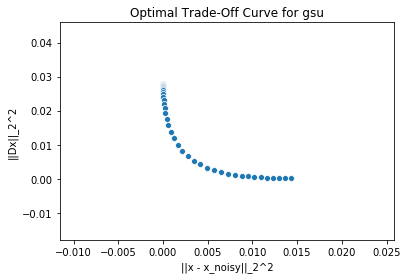
\includegraphics[scale=0.6]{gsu_optimal_trade_off.png}
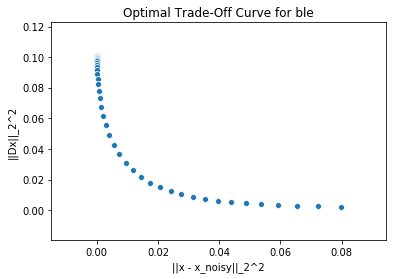
\includegraphics[scale=0.6]{ble_optimal_trade_off.png}
\caption{Plot of optimal trade-off curve for each of our subsytems. The plot are both generated using a geometric (logspace) sweep over $\mu \in [1e-4, 25)$.}
\label{fig:optimal_trade_off_curces}
\end{figure}

\begin{figure}[!ht]
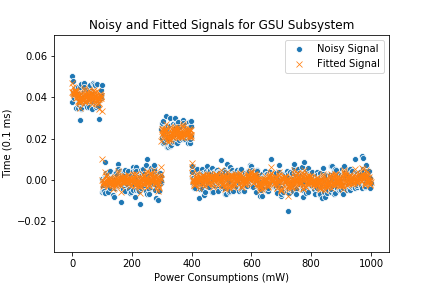
\includegraphics[scale=0.6]{gsu_subsystem_plot.png}
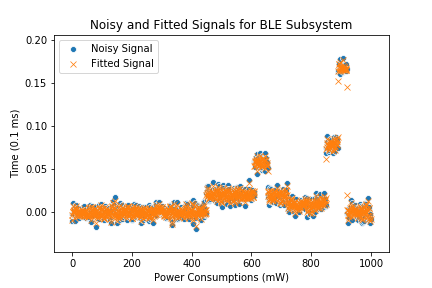
\includegraphics[scale=0.6]{ble_subsystem_plot.png}
\caption{Plot of the received signal as well as the fitted signal for GSU and BLE subsystems..}
\label{fig:signal_and_fit_curves}
\end{figure}

  \includepdf[
      %% Include all pages of the PDF
      pages=-,
      %% make this page have the usual page style
      %% (you can change it to plain etc). By default pdfpages
      %% sets the pagecommand to \pagestyle{empty}
      pagecommand={\pagestyle{headings}}]
  %% The pdf file itself
  {MidtermCode.pdf}









\end{document}
